%! Author = kubec
%! Date = 27.03.2024

% Preamble
\documentclass[11pt]{article}

% Packages
\usepackage{amsmath}
\usepackage{mathtools}
\usepackage{ragged2e}
\usepackage [utf8]{inputenc}
\usepackage{blindtext}
\usepackage{wrapfig}
\usepackage{xcolor}
\usepackage {polski}
\usepackage{multicol}
\usepackage[a4paper, total={5.7in, 8in}]{geometry}
\usepackage{graphicx}
\usepackage{amstex}
\usepackage{csvsimple}
\usepackage{changepage}
\usepackage{enumitem}
\usepackage[english]{babel}
\usepackage{biblatex}
\usepackage{caption}
\usepackage{indentfirst}

\newenvironment{changemargin}[2]{%
    \begin{list}{}{%
        \setlength{\topsep}{0pt}%
        \setlength{\leftmargin}{#1}%
        \setlength{\rightmargin}{#2}%
        \setlength{\listparindent}{\parindent}%
        \setlength{\itemindent}{\parindent}%
        \setlength{\parsep}{\parskip}%
    }%
        \item[]}{\end{list}}

% Document
\begin{document}
    \begin{flushright}
        \large{
            Igor Czerwiec - 277680\\
            Filip Kubecki - 272655
        }\\
    \end{flushright}
    \begin{center}
        \large{Fizyka 3.1}\\
        \vspace{2mm}
        \LARGE{\textbf{Wyznaczanie stałej Planca na podstawie charakterystyki diody elektroluminescencyjnej}}\\
        \vspace{3mm}
        \huge{Nr ćwiczenia: 48}\\
        \vspace{1cm}
    \end{center}
    \begin{flushright}
        \large{
            Data wykonania ćwiczenia: 11.04.2024 r.\\
            Data oddania sprawozdania: 17.04.2024 r.
        }\\
    \end{flushright}
    \vspace{1cm}
    \section{Wstęp}
    \textbf{Wykorzystane przyrządy pomiarowe:}
    \begin{itemize}
        \itemsep0em
        \item Multimetr Sanwa CD771
        \item Multimetr Jenit JT890
        \item Monochromator
    \end{itemize}
    \subsection*{Przebieg doświadczenia}
    \subsubsection*{Pomiar charakterystyki napięciowo prądowej diody}
    \begin{center}
        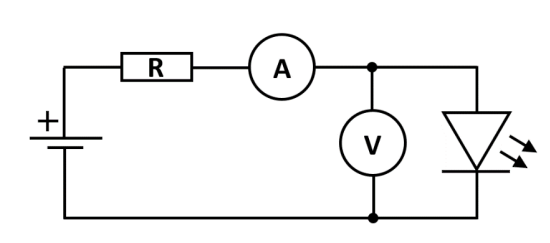
\includegraphics[scale = 0.45]{"F:/Projekty Intellij/Text/Fizyka3.1/48/Img/dioda.png"}
    \end{center}
    Przy pomocy multimetrów cyfrowych zmierzono charakterystykę prądowo-napięciową
    dla czerwonej/żółtej/zielonej oraz niebieskiej diody elektroluminescencyjnej. Pomiary były wykonywane co
    50[mV] od momentu przewodzenia diody do momentu osiągnięcia końca zakresu układu zasilającego.
    \subsubsection*{Pomiar długości fali diody}
    Przy pomocy monochromatora ustalono długość fali dla kolejnych diod:
    \begin{itemize}
        \item dla diody czerwonej - 630 [nM]
        \item dla diody żółtej - 590 [nM]
        \item dla diody niebieskiej - 460 [nM]
        \item dla diody zielonej - 560 [nM]
    \end{itemize}
    Wyniki te pokrywają się, w granicach niepewności pomiarowych, z
    danymi producentów diod elektroluminescencyjnych. Zakresy długości fali dla diod według producentów:
    \begin{itemize}
        \item dla diody czerwonej - od 627 [nM] do 780 [nM]
        \item dla diody żółtej - od 566 [nM] do 589 [nM]
        \item dla diody niebieskiej - od 436 [nM] do 495 [nM]
        \item dla diody zielonej - od 495 [nM] do 566 [nM]
    \end{itemize}

    \subsection*{Zastosowana teoria}
    Dioda elektroluminescencyjna to urządzenie elektryczne oparte na
    złączu p-n, czyli połączeniu półprzewodnika typu n (z przewagą elektronów) i
    półprzewodnika typu p (z przewagą dziur elektronowych). Gdy do takiego złącza nie
    jest przyłożone napięcie, w jego środkowej części w wyniku rekombinacji elektronów i
    dziur tworzy się warstwa zaporowa o znikomej ilości wolnych ładunków, uniemożliwiająca
    swobodny przepływ ładunku. Jeśli złącze zostanie spolaryzowane w kierunku przewodzenia
    (poprzez przyłożenie napięcia) elektrony w półprzewodniku typu n i dziury w półprzewodniku
    typu p zaczną być przyciągane w kierunku warstwy zaporowej, powodując jej zmniejszanie. \\
    \indent Przy wystarczająco dużym napięciu (napięcie odpowiadające barierze potencjału) warstwa zaporowa
    zanika; od tego momentu prąd płynie swobodnie i natężenie rośnie wraz z napięciem w sposób
    liniowy zgodnie z prawem Ohma. Rekombinacja w obszarze złącza zaczyna wtedy zachodzić w sposób
    ciągły. Rekombinacja powoduje oddanie przez elektron energii równej różnicy między pasmem
    przewodnictwa a pasmem walencyjnym poprzez emisję fotonu (rekombinacja promienista). Energia
    ta jest w przybliżeniu równa iloczynowi napięcia odpowiadającemu barierze potencjału i ładunku elektronu:
    \begin{gather*}
        E\approx U_B\cdot e
    \end{gather*}
    {\footnotesize
        \begin{itemize}
            \item[] $E$ - energia emitowanego fotonu,
            \item[] $U_B$ - napięcie odpowiadające barierze potencjału,
            \item[] $e$ - ładunek elementarny,
        \end{itemize}}
    \noindent Energia fotonu jest powiązana z długością fali promieniowania w następujący sposób:
    \begin{gather*}
        E=h\cdot\frac{c}{\lambda}
    \end{gather*}
    {\footnotesize
        \begin{itemize}
            \item[] $h$ - stałą Planca,
            \item[] $c$ - prędkość światła,
            \item[] $\lambda$ - długość fali,
        \end{itemize}}
    \noindent Po przekształceniu otrzymujemy:
    \begin{gather*}
        h=\frac{e}{c}\cdot U_B\cdot\lambda
    \end{gather*}
    \indent Stałą Plancka h możemy więc wyznaczyć mierząc
    napięcie odpowiadające barierze potencjału diody elektroluminescencyjnej
    oraz długość fali emitowanego przez nią światła.

    \section{Dane}
    %    Dioda czerwona
    \begin{center}
        \small\textbf{Wyniki dla diody czerwonej}
    \end{center}
    \begin{center}
        \csvreader[tabular = |c|c|c|c|c|,
            table head = \hline \textbf{U[V]} & \textbf{I[mA]} & \textbf{u(U)[V]} & \textbf{u(I)[mA]}\\\hline,
            late after line = \\\hline
        ]{Dane/RedDiodeData.csv}{}{
            \csvcoli & \csvcolii & \csvcolv & \csvcolvi
        }
    \end{center}
    \newpage
    %    Dioda żółta
    \begin{center}
        \small\textbf{Wyniki dla diody żółtej}
    \end{center}
    \begin{center}
        \csvreader[tabular = |c|c|c|c|c|,
            table head = \hline \textbf{U[V]} & \textbf{I[mA]} & \textbf{u(U)[V]} & \textbf{u(I)[mA]}\\\hline,
            late after line = \\\hline
        ]{Dane/YellowDiodeData.csv}{}{
            \csvcoli & \csvcolii & \csvcolv & \csvcolvi
        }
    \end{center}
    %    Dioda zielona
    \begin{center}
        \small\textbf{Wyniki dla diody zielonej}
    \end{center}
    \begin{center}
        \csvreader[tabular = |c|c|c|c|c|,
            table head = \hline \textbf{U[V]} & \textbf{I[mA]} & \textbf{u(U)[V]} & \textbf{u(I)[mA]}\\\hline,
            late after line = \\\hline
        ]{Dane/GreenDiodeData.csv}{}{
            \csvcoli & \csvcolii & \csvcolv & \csvcolvi
        }
    \end{center}
    \newpage
    %    Dioda niebieska
    \begin{center}
        \small\textbf{Wyniki dla diody niebieskiej}
    \end{center}
    \begin{center}
        \csvreader[tabular = |c|c|c|c|c|,
            table head = \hline \textbf{U[V]} & \textbf{I[mA]} & \textbf{u(U)[V]} & \textbf{u(I)[mA]}\\\hline,
            late after line = \\\hline
        ]{Dane/BlueDiodeData.csv}{}{
            \csvcoli & \csvcolii & \csvcolv & \csvcolvi
        }
    \end{center}

    \section{Obliczenia}
    \noindent Niepewność bezwzględną multimetru wyliczamy ze wzoru:
    \begin{gather*}
        \Delta=a\%\cdot rdg+c\cdot dgt
    \end{gather*}
    {\footnotesize
        \begin{itemize}
            \item[] $a,c$ - współczynniki podawane przez producenta,
            \item[] $rdg$ - wartość odczytana z miernika,
            \item[] $dgt$ - najmniejsza możliwa do odczytania wartość na wykorzystanym zakresie,
        \end{itemize}}
    \noindent Przykładowo dla pomiaru napięcia barierę potencjału diody wyliczamy ze wzoru:
    \begin{gather*}
        U_B=-\frac{b}{a}
    \end{gather*}
    \newpage
    \noindent Przykładowo dla diody niebieskiej:
    \begin{gather*}
        U_B=-\frac{b}{a}=-\frac{-143.059950}{50.063309}=2.857581[V]
    \end{gather*}
    Niepewność obliczania bariery potencjału obliczamy z wzoru na niepewność złożoną:
    \begin{gather*}
        u_c(U_B)=\sqrt{((\frac{\partial f(U_B)}{\parial a})\cdot u(a))^2+((\frac{\partial f(U_B)}{\parial b})\cdot u(b))^2}=\\
        =\sqrt{((\frac{b}{a^2})\cdot u(a))^2+((\frac{-1}{a})\cdot u(b))^2}
    \end{gather*}
    Przykładowo dla diody niebieskiej:
    \begin{gather*}
        u_c(U_B)=\sqrt{((\frac{-143.059950}{50.063309^2})\cdot 5.041035)^2+((\frac{-1}{50.063309})\cdot 15.263963)^2}=\\
        =0.4192298[V]\approx 0.42[V]
    \end{gather*}
    Stałą Planca wyznaczamy ze wzoru:
    \begin{gather*}
        h=\frac{e}{c}\cdot U_B\cdot\lambda
    \end{gather*}
    Przykładowo dla diody niebieskiej:
    \begin{gather*}
        h=\frac{1.602\cdot 10^{-19}[C]}{299792458[\frac{m}{s}]}\cdot 2.857581[V]\cdot 4.6\cdot 10^{-7}[m]=7.024995\cdot 10^{-34}[J\cdot s]
    \end{gather*}
    Niepewność obliczania stałej Planca obliczamy z wzoru na niepewność złożoną:
    \begin{gather*}
        u_c(h)=\sqrt{(\frac{\partial f(h)}{\partial U_B}\cdot u(U_B))^2+(\frac{\partial f(h)}{\partial \lambda}\cdot u(\lambda))^2}=\\
        =\sqrt{(\frac{e}{c}\cdot\lambda\cdot u(U_B))^2+(\frac{e}{c}\cdot U_B\cdot u(\lambda))^2}
    \end{gather*}
    Przykładowo dla diody niebieskiej:
    \begin{gather*}
        u_c(h)=\\
        =\sqrt{(\frac{1.602\cdot 10^{-19}[C]}{299792458[\frac{m}{s}]}\cdot 4.6\cdot 10^{-7}[m]\cdot 0.42[V])^2+
            (\frac{1.602\cdot 10^{-19}[C]}{299792458[\frac{m}{s}]}\cdot 2.857[V]\cdot 5.77\cdot 10^{-9})^2[m]}=\\
        =1.034387\cdot 10^{-34}[J\cdot s]=1.1\cdot 10^{-34}[J\cdot s]
    \end{gather*}

    \section{Wyniki}
    \subsection*{Wykres zależności napięcia od natężenie prądu elektrycznego dla kolejnych diod}
    \begin{center}
        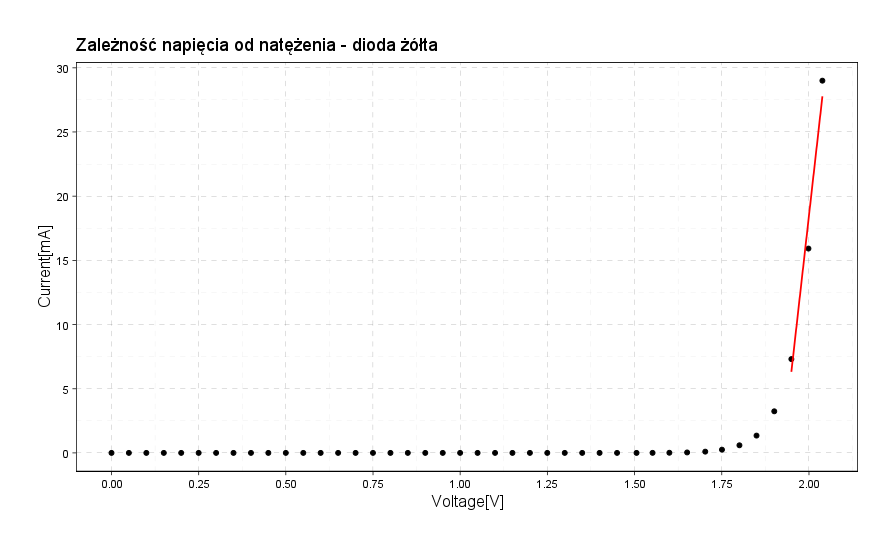
\includegraphics[scale = 0.45]{"F:/Projekty Intellij/Text/Fizyka3.1/48/Img/Rplot01.png"}
    \end{center}
    \begin{center}
        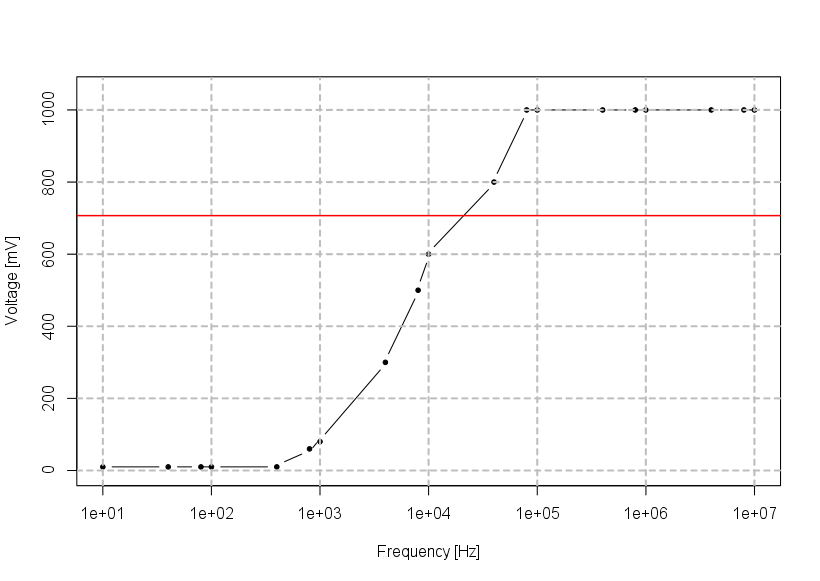
\includegraphics[scale = 0.45]{"F:/Projekty Intellij/Text/Fizyka3.1/48/Img/Rplot02.png"}
    \end{center}
    \begin{center}
        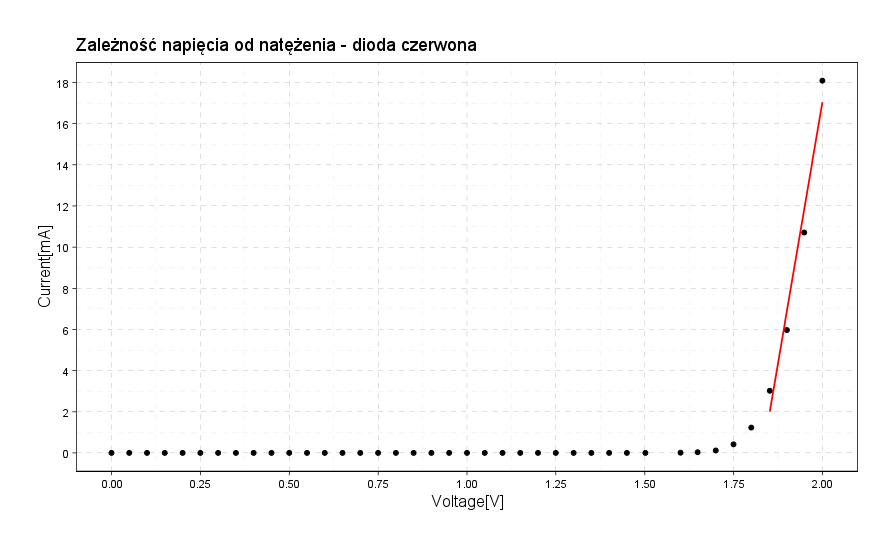
\includegraphics[scale = 0.45]{"F:/Projekty Intellij/Text/Fizyka3.1/48/Img/Rplot03.png"}
    \end{center}
    \begin{center}
        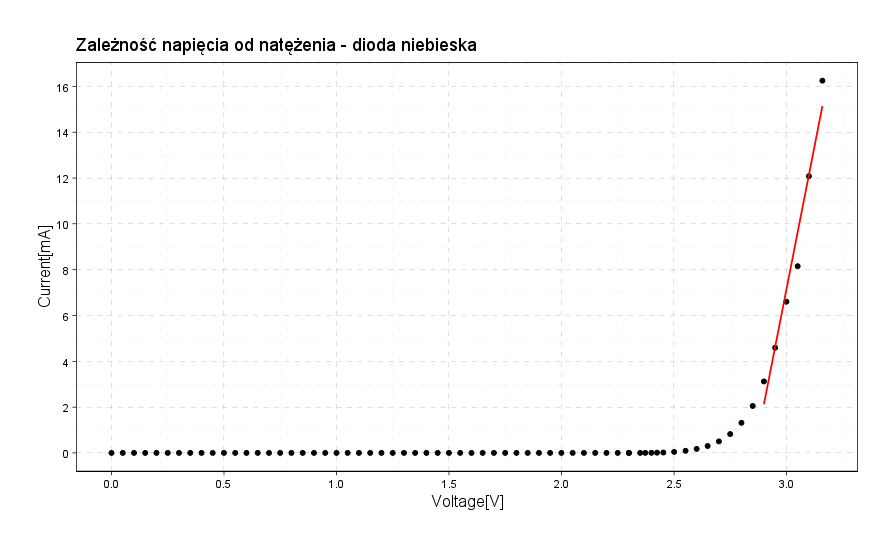
\includegraphics[scale = 0.45]{"F:/Projekty Intellij/Text/Fizyka3.1/48/Img/Rplot04.png"}
    \end{center}

    \subsection*{Bariery potencjału oraz stałe planca dla kolejnych diod}
    Dla referencji tablicowa wartość stałej Planca:
    \begin{gather*}
        h=6.62607015\cdot 10^{-34}[J\cdot s]
    \end{gather*}
    \begin{center}
        \csvreader[tabular = |c|c|c|c|c|,
            table head = \hline \textbf{Typ diody} & \textbf{$U_B$[V]} & \textbf{$u(U_B)$[V]} & \textbf{h[Js]} & \textbf{u(h)[Js]}\\\hline,
            late after line = \\\hline
        ]{Dane/Wyniki.csv}{}{
            \csvcoli & \csvcolii & \csvcoliii & \csvcoliv & \csvcolv
        }
    \end{center}

    \section{Wnioski}
    \indent Na podstawie eksperymentu udało się wyznaczyć stałą planca dla każdej z diod.
    Dla diody zielonej wartość tak nie mieści się w zakresie jej niepewności pomiarowej.
    Dla pozostałych diod wyniki zawierały się w przedziale niepewności pomiarowych jednak niepewność względna
    dla tych pomiarów potrafiła wynosić nawet $\approx 26\%$ (dla diody żółtej).\\
    \indent Tak duża wartość niepewności oraz tak mało dokładne wyniki wynikają bezpośrednio z metody pomiarowej.
    Barierę potencjału dla kolejnych diod wyliczano na podstawie ostatnich 3 do 6 pomiarów które układały się w funkcje liniową.
    Z powodu tak małej ilości punktów regresja liniowa nie była dokładna co zwiększyło znacząco jej niepewność.\\
    \indent Aby poprawić wyniki doświadczenia należałoby zwiększyć ilość punktów pomiarowych do np 50 co wydłużyłoby jednak znacząco
    czas przeprowadzania doświadczenia. Możnabyłoby też wykonywać pomiary od końca zakresu z mniejszym skokiem napięcia
    (np. 10 [mV]). Nie pozwoliłoby to na uzyskanie pełnej charakterystyki napięciowo-prądowej dla diod ale pozwoliłoby
    na dokładniejsze wyznaczenie stałej Planca.

    %Bibliografia
    \vfill
    \footnotesize
    \begin{thebibliography}{9}
        \bibitem{texbook1}
        https://lpf.wppt.pwr.edu.pl/instrukcje/cwn048.pdf
        \bibitem{texbook2}
        https://lpf.wppt.pwr.edu.pl/pomoce-dydaktyczne.php
        \bibitem{texbook3}
        https://www.wolframalpha.com/
        \bibitem{texbook4}
        https://en.wikipedia.org/wiki/Planck-constant
        \bibitem{texbook5}
        https://www.growtent.pl/Barwa-swiatla-LED-oraz-HPS-do-doswietlania-roslin-blog-pol-1494238911.html
    \end{thebibliography}
\end{document}